\documentclass[twoside,11pt]{article}

% Any additional packages needed should be included after jmlr2e.
% Note that jmlr2e.sty includes epsfig, amssymb, natbib and graphicx,
% and defines many common macros, such as 'proof' and 'example'.
%
% It also sets the bibliographystyle to plainnat; for more information on
% natbib citation styles, see the natbib documentation, a copy of which
% is archived at http://www.jmlr.org/format/natbib.pdf

\usepackage{jmlr2e}
\usepackage[cachedir=.,finalizecache]{minted}
\usepackage[utf8]{inputenc} % allow utf-8 input
\usepackage{graphicx}
\usepackage{caption}
\usepackage{subcaption}
\usepackage{stmaryrd}
\usepackage[colorinlistoftodos]{todonotes}
\newcommand{\aurelien}[1]{\todo[inline,caption={},color=orange!40]{{\it Aurelien:~}#1}}
\newcommand{\william}[1]{\todo[inline,caption={},color=blue!40]{{\it William:~}#1}}
%\renewcommand{\aurelien}[1]{}
%\renewcommand{\william}[1]{}


\graphicspath{{images/}}

% Definitions of handy macros can go here

\newcommand{\dataset}{{\cal D}}
\newcommand{\fracpartial}[2]{\frac{\partial #1}{\partial  #2}}

% Heading arguments are {volume}{year}{pages}{submitted}{published}{author-full-names}

\jmlrheading{}{}{}{}{}{William de Vazelhes and CJ Carey and Yuan Tang and Nathalie Vauquier and Aur\'elien Bellet}

% Short headings should be running head and authors last names

\ShortHeadings{metric-learn: Metric Learning Algorithms in Python}{de Vazelhes, Carey, Tang, Vauquier and Bellet}
\firstpageno{1}

\begin{document}

\title{metric-learn: Metric Learning Algorithms in Python}

\author{\name William de Vazelhes \email william.de-vazelhes@inria.fr \\
       \addr INRIA, France
       \AND
       \name CJ Carey \email perimosocordiae@gmail.com \\
       \addr Google LLC, United States
       \AND
       \name Yuan Tang \email terrytangyuan@gmail.com \\
       \addr Ant Financial, United States
       \AND
       \name Nathalie Vauquier \email nathalie.vauquier@inria.fr \\
       \addr INRIA, France
       \AND
       \name Aur\'elien Bellet \email aurelien.bellet@inria.fr \\
       \addr INRIA, France
       }

\editor{}

\maketitle

\begin{abstract}%   <- trailing '%' for backward compatibility of .sty file
\texttt{metric-learn} is an open source Python package implementing supervised and weakly-supervised distance metric learning algorithms. As part of \texttt{scikit-learn-contrib}, it provides a unified interface compatible with \texttt{scikit-learn} which allows to easily perform cross-validation, model selection, and pipelining with other machine learning estimators. \texttt{metric-learn} is thoroughly tested and available on PyPi under the MIT licence.
%The source code is available online at \url{http://github.com/scikit-learn-contrib/metric-learn}, as well as the documentation at \url{http://metric-learn.github.io/metric-learn/}.
\end{abstract}

\begin{keywords}
  Machine Learning, Python, Metric Learning, Scikit-learn
\end{keywords}

\section{Introduction}

Many approaches in machine learning require a measure of distance between data
points. Traditionally, practitioners would choose a standard distance metric
(Euclidean, City-Block, Cosine, etc.) using a priori knowledge of the
domain. However, it is often difficult to design metrics that are well-suited
to the particular data and task of interest.
% \todo[inline]{probably need to add a sentence explaining what is meant by weak supervision}
Distance metric learning, or simply metric learning \citep{Bellet15}, aims at
automatically constructing task-specific distance metrics from data. A key advantage of metric learning is that it can be applied beyond the standard supervised learning setting (data points associated with labels), in situations where only weaker forms of supervision are available (e.g., pairs of points that should be similar/dissimilar). The learned distance metric can be used to perform retrieval tasks such as finding elements (images, documents) of a database that are semantically closest to a query element. It can also be plugged into other machine learning algorithms, for instance to improve the accuracy of nearest neighbors models (for classification, regression, anomaly detection...) or to bias the clusters found by clustering algorithms towards the intended semantics. Finally, metric learning can be used to perform dimensionality reduction.
These use-cases highlight the importance of integrating metric learning with the rest of the machine learning pipeline and tools.
% \todo[inline]{quick presentation of the package: implements several algorithms, with sklearn-compatible API for model selection, model evaluation, pipelining with other estimators. makes metric-learn stands out from other packages (maybe mention a few of them), in particular in the case of weakly supervised algorithms}

\texttt{metric-learn} is an open source package for metric learning in Python, which implements many popular metric-learning algorithms with different levels of supervision through a unified interface.
%\footnote{This makes \texttt{metric-learn} stand out from other packages, like \texttt{PyDML} (\url{https://github.com/jlsuarezdiaz/pyDML}) which focuses on supervised metric learning algorithms.}
% (not only class supervision, unlike most packages are focused on, including another package for metric learning in Python, \texttt{PyDML})
% , which is one interesting feature allowed by the metric learning paradigm. 
Its API is compatible with \texttt{scikit-learn} \citep{scikit-learn}, a prominent machine learning library in Python. This allows for streamlined model selection, evaluation, and pipelining with other estimators.
Other packages for metric learning already exist, however, they have a different focus: \texttt{DistLearn}\footnote{\url{https://www.cs.cmu.edu/~liuy/distlearn.htm}} and \texttt{pyDML}\footnote{\url{http://github.com/jlsuarezdiaz/pydml}} contain almost only fully supervised or unsupervised metric learning algorithms, and \texttt{pytorch-metric-learning}\footnote{\url{http://github.com/KevinMusgrave/pytorch-metric-learning}} is focused on deep metric learning, using the pytorch framework.
% The project is developed collaboratively through GitHub, its code is thoroughly tested using continuous integration tools. It was recently included to \texttt{scikit-learn-contrib}, which hosts high-quality \texttt{scikit-learn}-compatible projects.\footnote{\url{https://github.com/scikit-learn-contrib/scikit-learn-contrib}}
%\aurelien{decide if we include or not a few sentences on positioning wrt other packages}

%, which makes \texttt{metric-learn} stand out from other packages, like \texttt{PyDML} \footnote{\url{https://github.com/jlsuarezdiaz/pyDML}}, which mostly focuses on supervised metric learning algorithms.
% Acknowledgements should go at the end, before appendices and references
%The rest of this paper is organized as follows. We first present an overview of the package, followed by a more detailed description of the available algorithms. We then give more details about the API and the software architecture, in particular the compatibility with \texttt{scikit-learn}, and conclude with a discussion of future developments.

% \aurelien{we could put the presentation of metric learning and supervision as Sec 2, and put the implemented algorithms in the overview of the package section as Section 3}

\section{Background on Metric Learning} \label{metriclearning}

% \todo[inline]{comparison with other packages ? }
% Metric learning problems fall into two main categories depending on the type
% of supervision available about the training data:

% \begin{itemize}
%     \item 
% - Supervised learning: the algorithm has access to
%   a set of data points, each of them belonging to a class (label) as in a
%   standard classification problem.
%   Broadly speaking, the goal in this setting is to learn a distance metric
%   that puts points with the same label close together while pushing away
%   points with different labels.
% - Weakly supervised learning: the
%   algorithm has access to a set of data points with supervision only
%   at the tuple level (typically pairs, triplets, or quadruplets of
%   data points). A classic example of such weaker supervision is a set of
%   positive and negative pairs: in this case, the goal is to learn a distance
%   metric that puts positive pairs close together and negative pairs far away.


% \end{itemize}


% \paragraph{General setting} Metric learning problems are generally formulated as an optimization problem where one seeks to find, on the training data $(x_0, ..., x_n)$, the parameters $\theta$ of a distance function $D_\theta(x_i, x_j)$ that optimize some desired objective function $\mathcal{L}_\theta(x_0, ..., x_n) = f(D_\theta(x_0, x_0), ..., D_\theta(x_0, x_n), ..., D_\theta(x_n, x_0), ..., D_\theta(x_n, x_n))$, hoping that this metric will generalize the desired propertie(s) on new incoming test data.

Metric learning is generally formulated as an optimization problem where one seeks to find the parameters of a distance function that minimize some objective function over the input data.
All algorithms currently implemented in \texttt{metric-learn} learn so-called Mahalanobis distances. Given a real-valued parameter matrix $L$ of shape \texttt{(n\_components, n\_features)} where \texttt{n\_features} is the
number of features describing the data, the associated Mahalanobis distance between two points $x$ and $x'$ is defined as $D_L(x, x') = \sqrt{(Lx-Lx')^\top(Lx-Lx')}$.
This is equivalent to Euclidean distance after linear transformation of the feature space defined by $L$.
Thus, if $L$ is the identity matrix, standard Euclidean distance is recovered.
Mahalanobis distance metric learning can thus be seen as learning a new
embedding space, with potentially reduced dimension \texttt{n\_components}.
Note that $D_L$ can also be written as $D_L(x, x') = \sqrt{(x - x')^\top M (x - x')}$, where we refer to $M = L^\top L$ as the Mahalanobis matrix.

% Strictly speaking, Mahalanobis distances are "pseudo-metrics": they satisfy
% three of the properties of a metric (non-negativity, symmetry, triangle inequality) but not
% necessarily the identity of indiscernibles.

% Mahalanobis distances can also be parameterized by a positive semi-definite 
% (PSD) matrix $M$:

% $ D(x, x') = \sqrt{(x-x')^\top M(x-x')}$

% Using the fact that a PSD matrix :math:`M` can always be decomposed as
% $M=L^\top L$ for some  :math:`L`, one can show that both
% parameterizations are equivalent. In practice, an algorithm may thus solve
% the metric learning problem with respect to either :math:`M` or :math:`L`.

% use t to put figure on top (preferred) Thanks ! 
\begin{figure}[t]
    \centering
    \begin{subfigure}[t]{0.12\textwidth} % "0.45" donne ici la largeur de l'image
        \centering 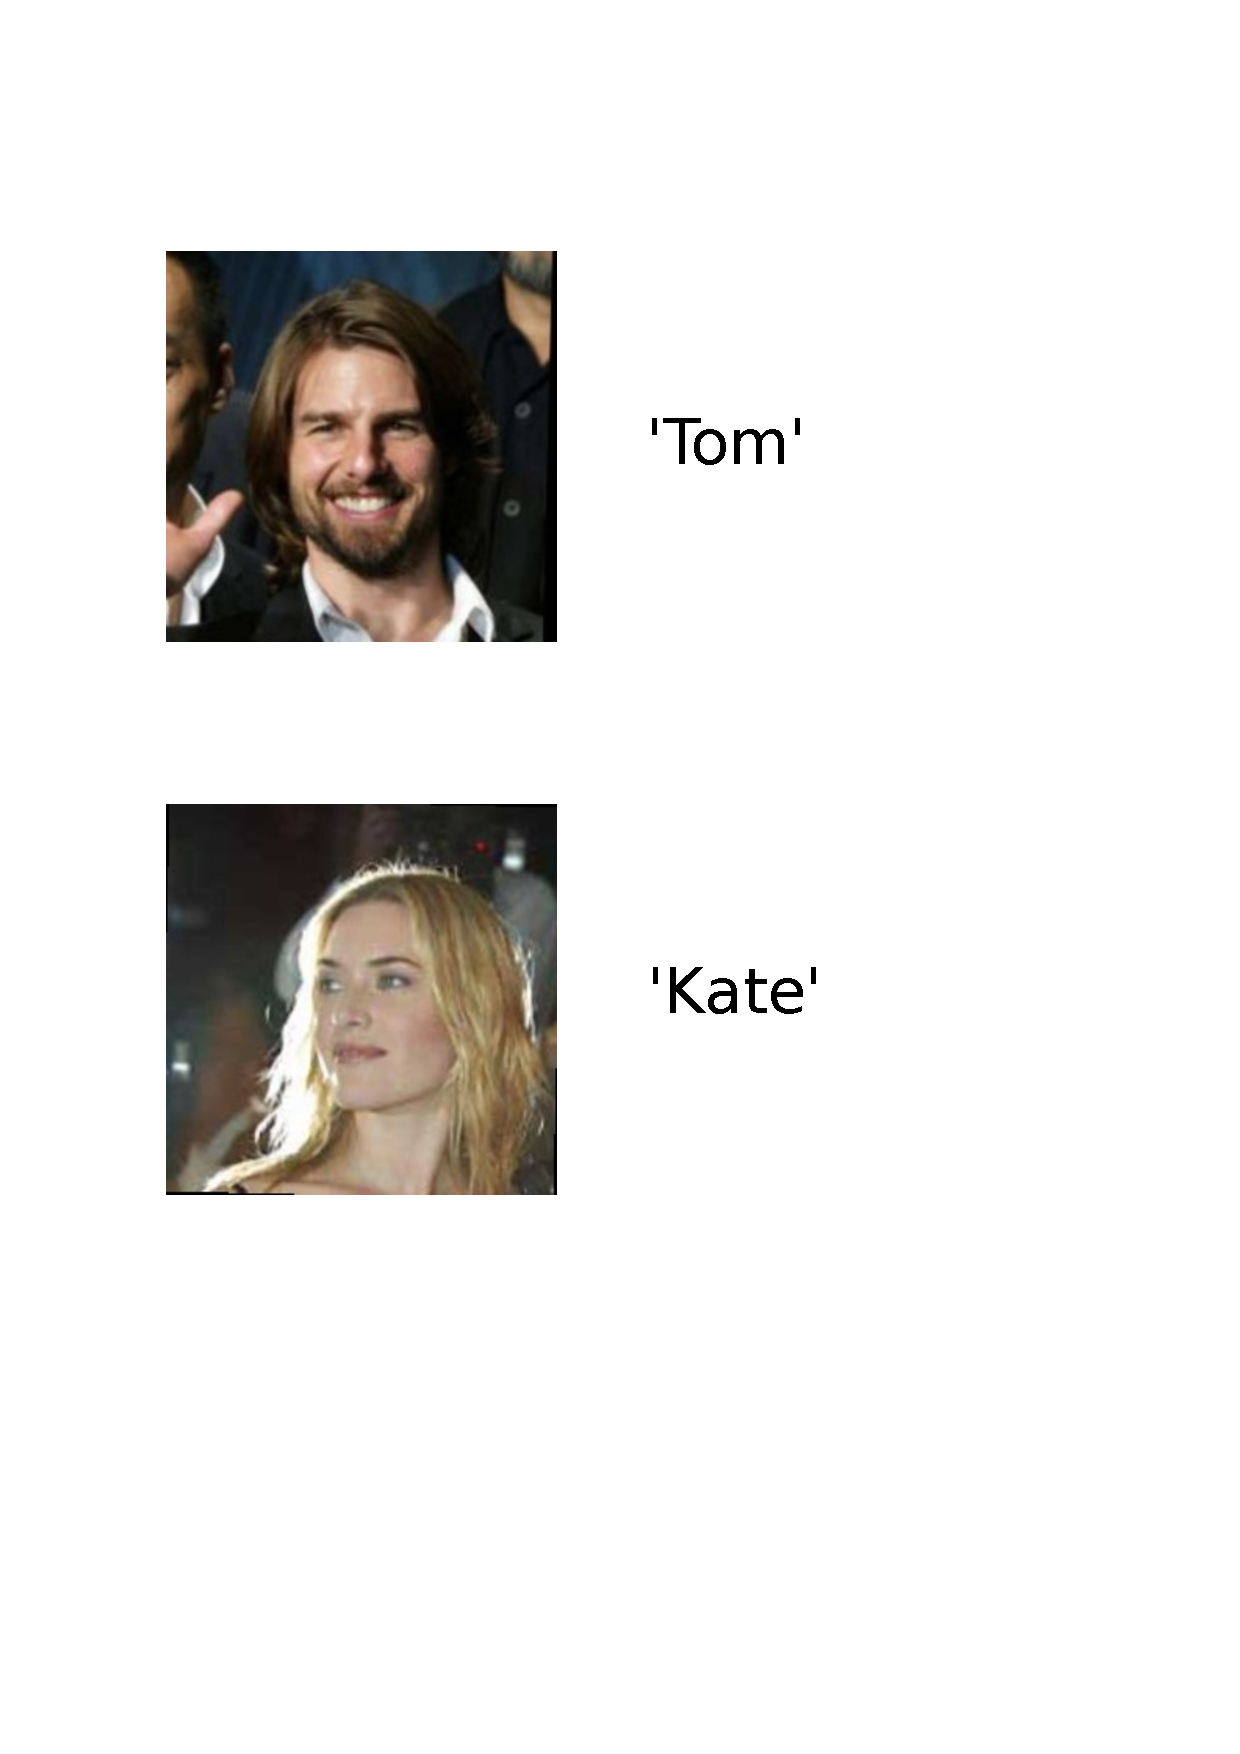
\includegraphics[scale=0.35]{labels.pdf}
        \caption{class}\label{fig:full}
    \end{subfigure}
    \begin{subfigure}[t]{0.20\textwidth}
        \centering 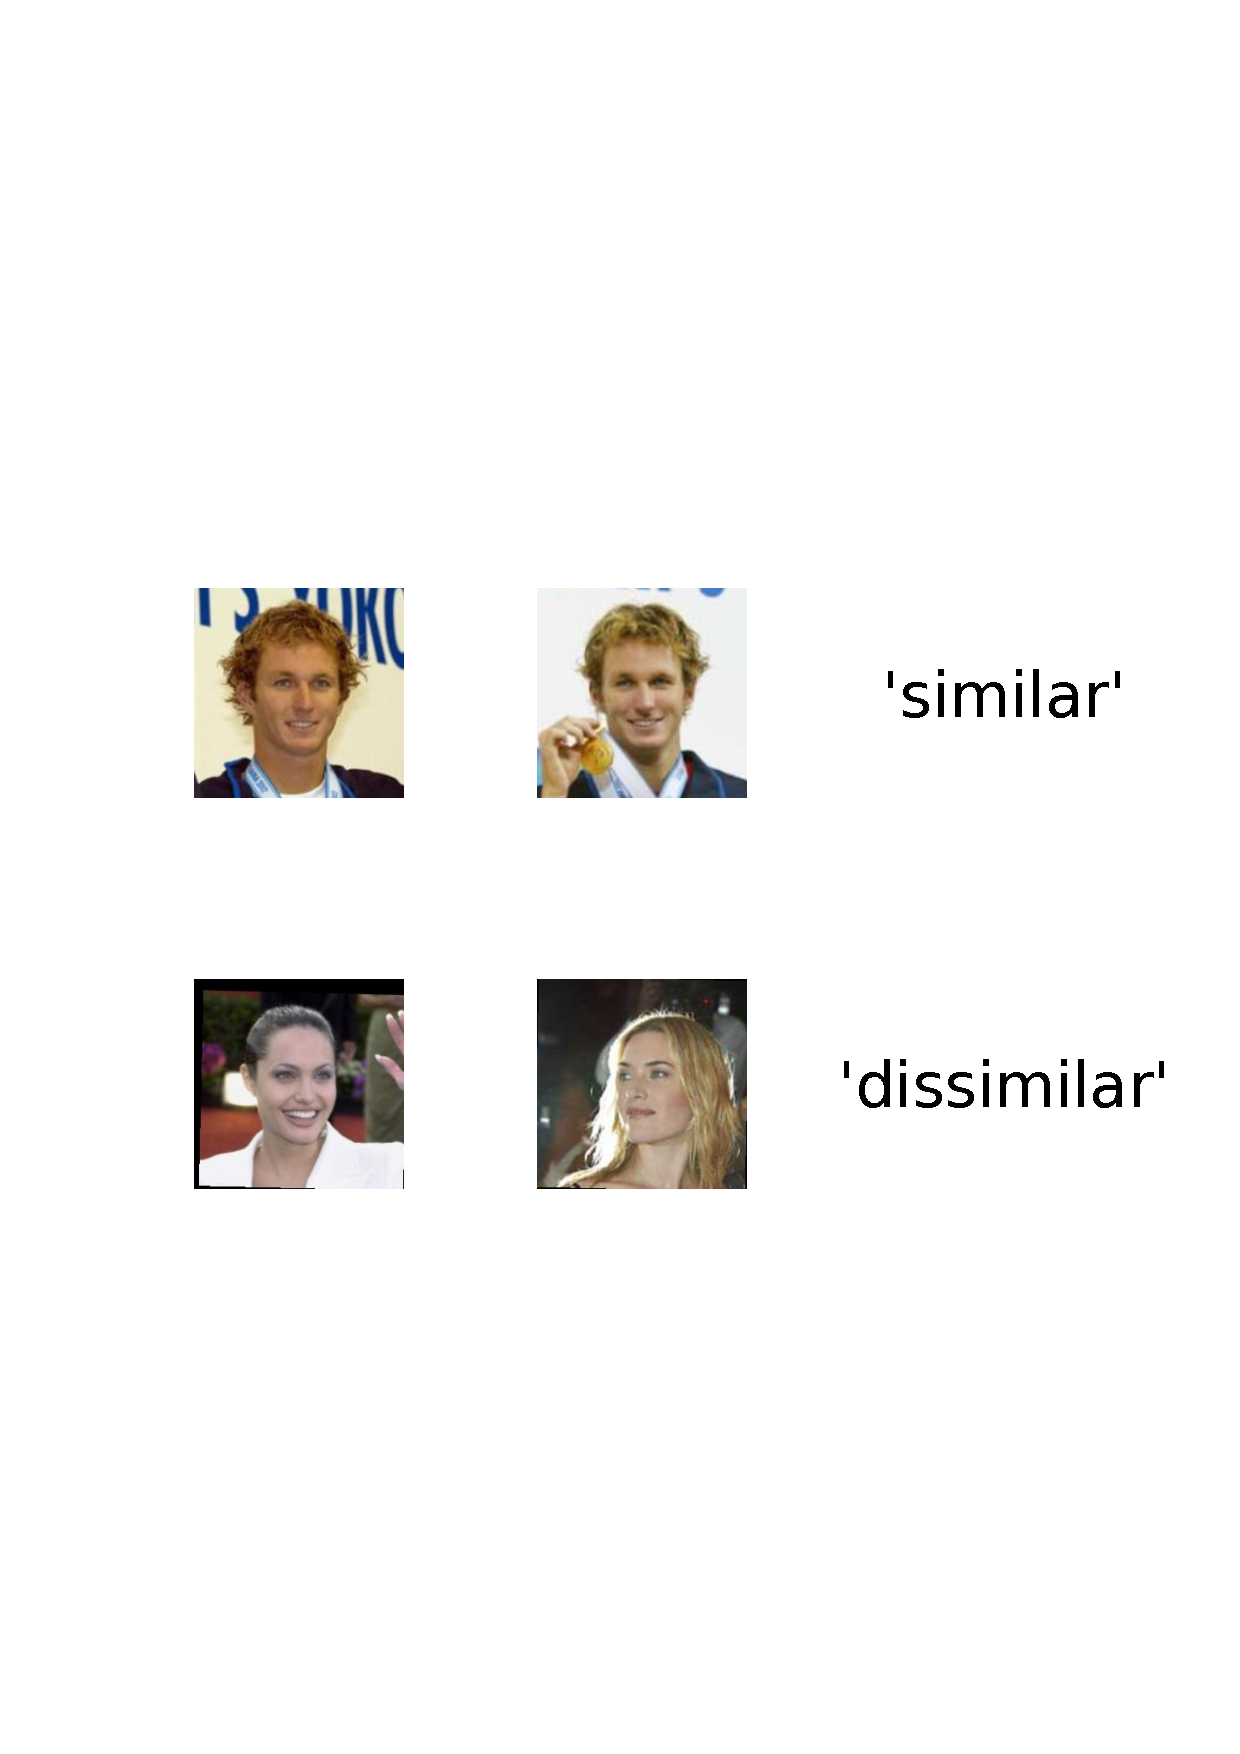
\includegraphics[scale=0.35]{pairs.pdf}
        \caption{pair}\label{fig:pairs}
    \end{subfigure}
    \begin{subfigure}[t]{0.31\textwidth}
        \centering 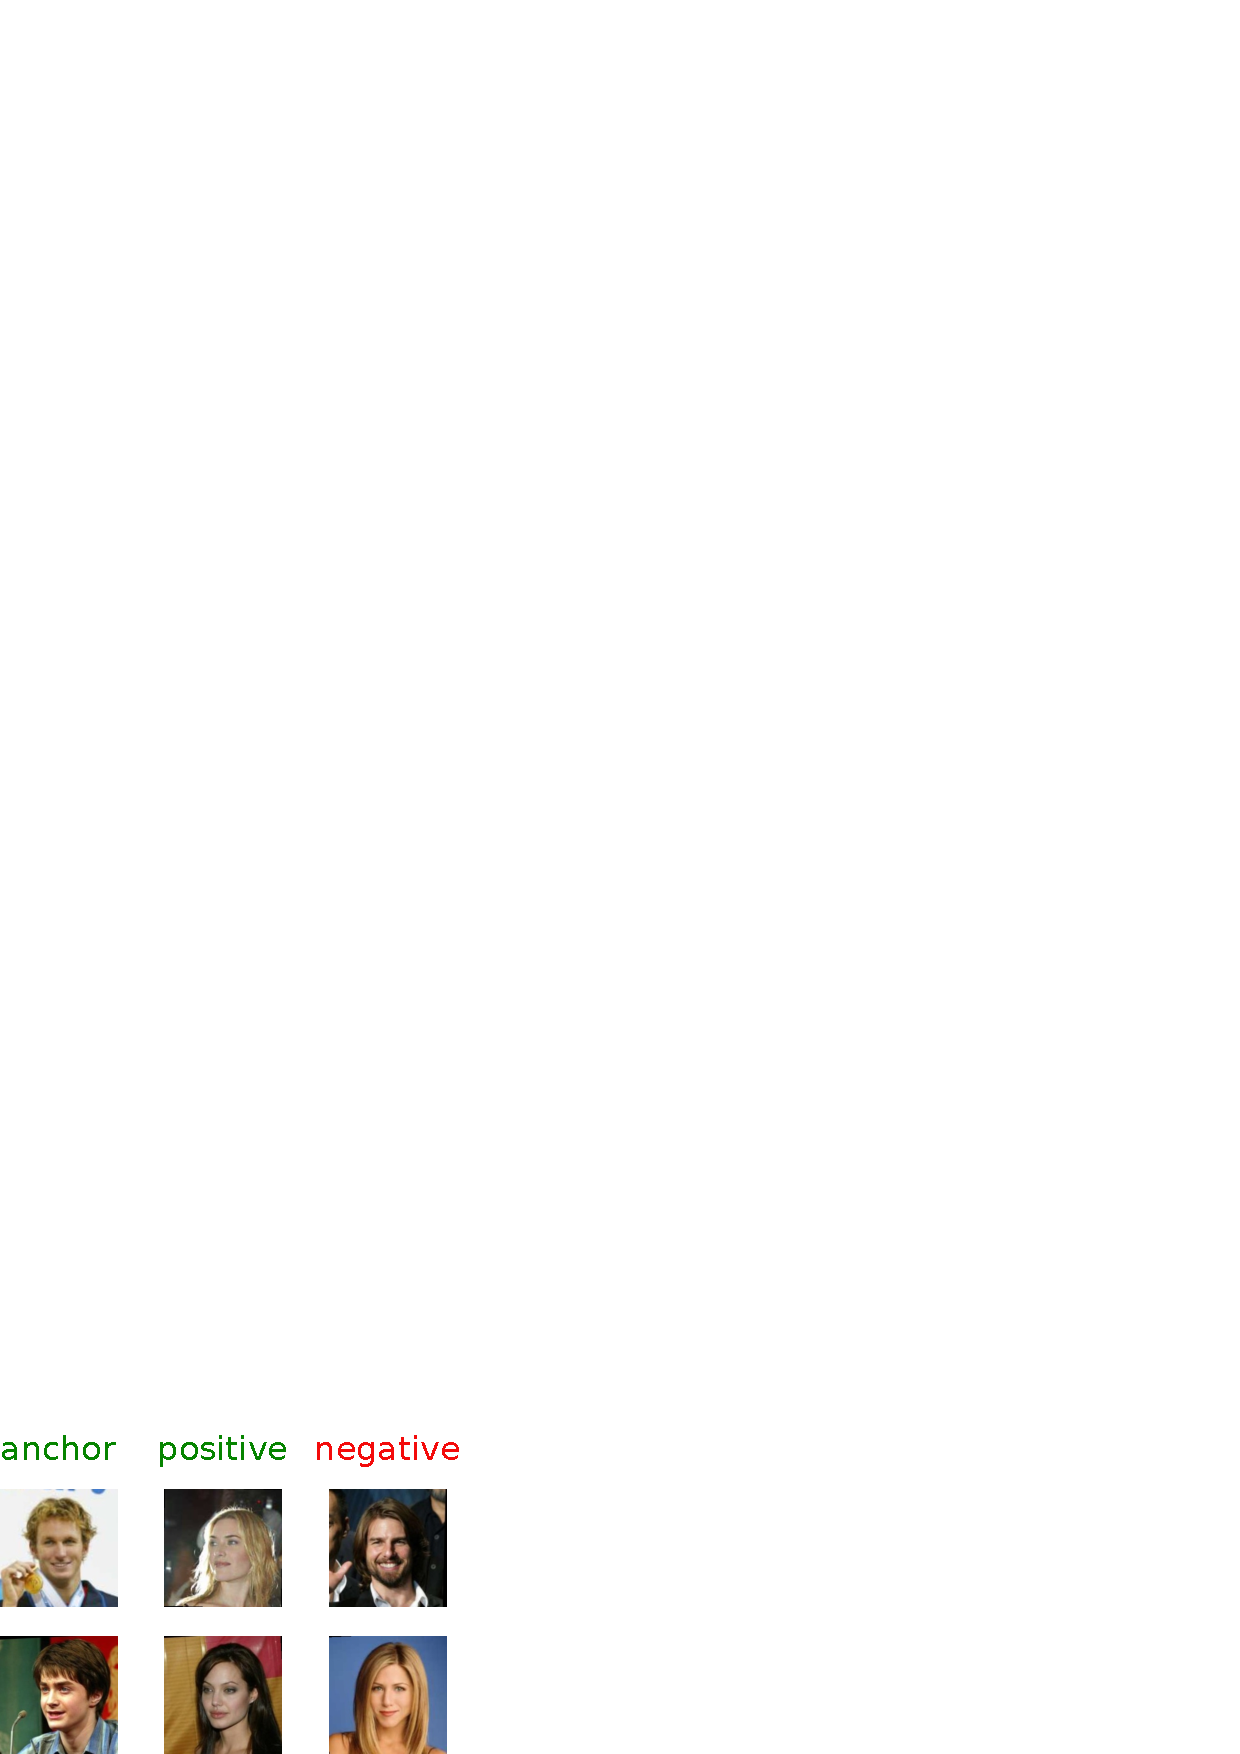
\includegraphics[scale=0.35]{triplets.pdf}
	\caption{triplet}\label{fig:triplets}
    \end{subfigure}
    \begin{subfigure}[t]{0.31\textwidth}
        \centering 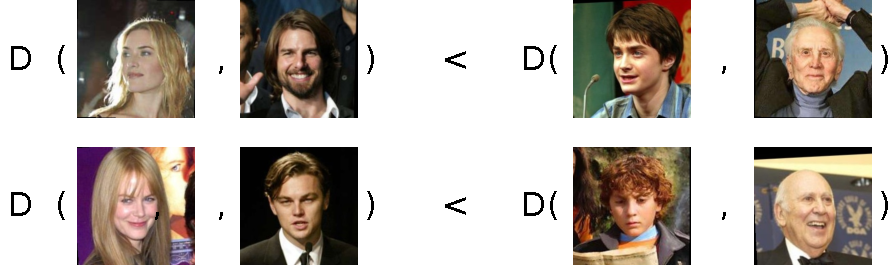
\includegraphics[scale=0.35]{quadruplets.pdf}
        \caption{quadruplet}\label{fig:quadruplets}
    \end{subfigure}
    \caption{Different types of supervision for metric learning %(\subref{fig:full}) Class supervision: make samples from the same label (here, identity) closer together than samples from different labels. (\subref{fig:pairs}) Pair supervision: make similar pairs (here, corresponding to the same person) to be closer than dissimilar pairs (different persons). (\subref{fig:quadruplets}) Quadruplet supervision: make leftmost pairs (here, people of similar age) closer than rightmost pairs (of bigger age difference).
    illustrated on face image data taken from the Labeled Faces in the Wild dataset \citep{Huang12}.}\label{fig:flowers}
\end{figure}

Metric learning algorithms can be categorized according to the form of data supervision they require to learn a metric.
\texttt{metric-learn} currently implements algorithms that fall into the following categories.
\emph{Supervised learners} learn from a dataset with one label per training example, aiming to bring together points from the same class while spreading points from different classes.
For instance, data points could be face images and the class could be the identity of the person (see Figure~\ref{fig:full}). 
% \todo[inline]{ces figures ne sont pas très vendeuses. je propose de faire une figure conceptuelle en prenant l'exemple des faces expliquant la différence entre le supervisé, les paires et les quadruplets. on peut s'inspirer de \url{http://cedric.cnam.fr/~thomen/papers/Law_ICCV_2013_QWise.pdf}}
% \begin{figure}[H]
% \centering
% \begin{subfigure}{.5\textwidth}
%   \centering
%   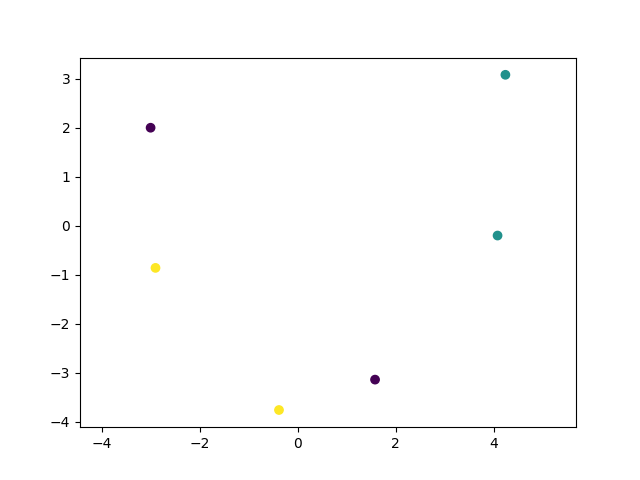
\includegraphics[width=.8\linewidth]{supervised_without_metric.png}
%   \caption{Original points, before metric learning}
%   \label{fig:sub1}
% \end{subfigure}%
% \begin{subfigure}{.5\textwidth}
%   \centering
%   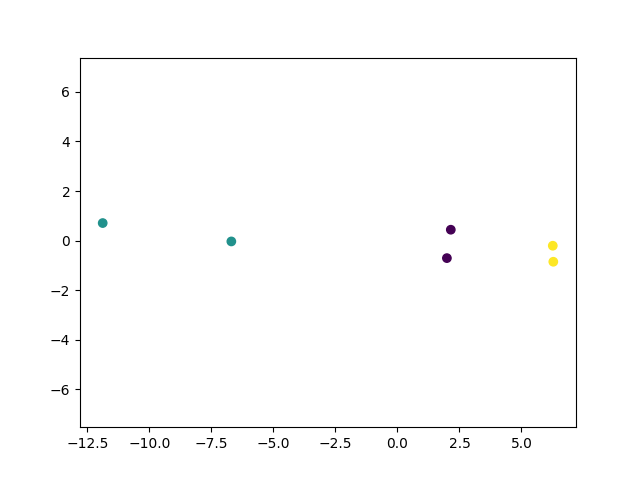
\includegraphics[width=.8\linewidth]{supervised_with_metric.png}
%   \caption{points after metric learning (ITML)}
%   \label{fig:sub2}
% \end{subfigure}
% \caption{Metric learning with pairwise constraints}
% \label{fig:test}
% \end{figure}
% \paragraph{Weakly Supervised Metric Learning algorithms}
% Weakly Supervised algorithms use less information than the previous algorithms: they only take tuple of points and possibly a corresponding label. See below for more concrete examples of algorithms learning on tuples.
\emph{Pair learners} require a set of pairs of points, with each pair labeled to indicate whether the two points are similar or not.
These methods aim to learn a metric that brings pairs of similar points closer together and pushes pairs of dissimilar points further away from each other.
Such supervision is often simpler to collect than class labels in applications when there are many labels. %, since annotators will only need to say whether images are similar or not, and will not have to assign a label in a huge list of those.
For instance, a human annotator can often quickly decide whether two face images correspond to the same person (Figure~\ref{fig:pairs}) while matching a face to its identity among many possible people may be difficult. 
% \begin{figure}[H]
% \centering
% \begin{subfigure}{.5\textwidth}
%   \centering
%   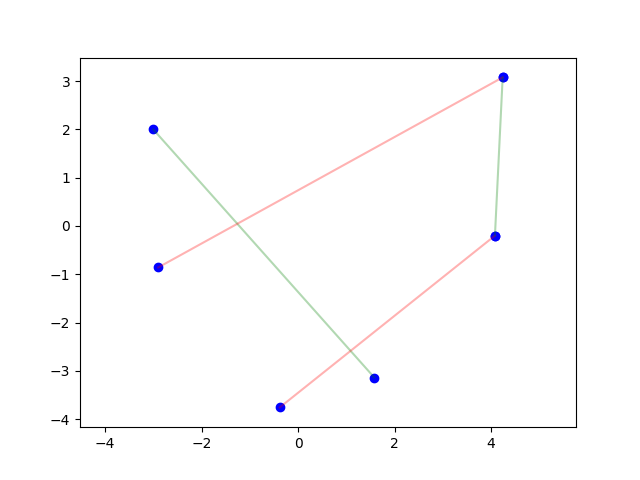
\includegraphics[width=.8\linewidth]{pairs_without_metric.png}
%   \caption{Original points, before metric learning}
%   \label{fig:sub1}
% \end{subfigure}%
% \begin{subfigure}{.5\textwidth}
%   \centering
%   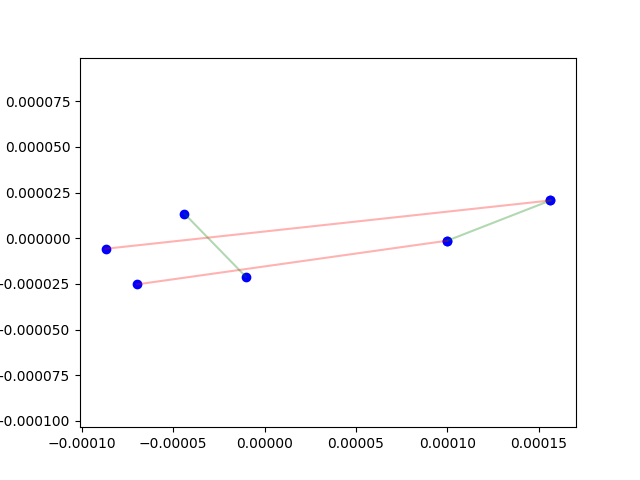
\includegraphics[width=.8\linewidth]{pairs_with_metric.png}
%   \caption{points after metric learning (ITML)}
%   \label{fig:sub2}
% \end{subfigure}
% \caption{Metric learning with pairwise constraints}
% \label{fig:test}
% \end{figure}
\emph{Triplet learners} consider 3-tuples of points and learn a metric that brings the anchor point and the positive point closer than the anchor and the negative point.
Finally, \emph{quadruplet learners} consider 4-tuples of points and aim to learn a metric that brings the two first points of each quadruplet closer than the two last points.
Both triplet learners and quadruplets learners can be used to learn a metric space in which closer points are more similar with respect to an attribute of interest, which may be continuous and difficult to annotate accurately (e.g., the age of a person on an image, see Figure \ref{fig:quadruplets}, or their hair color, see Figure \ref{fig:triplets}).
Quadruplet supervision is also used in problems with a class hierarchy.
%for instance, we want to learn a metric that puts closer together people from approximately the same age.


% \begin{figure}[h]
% \centering
%   \begin{subfigure}[b]\centering
%      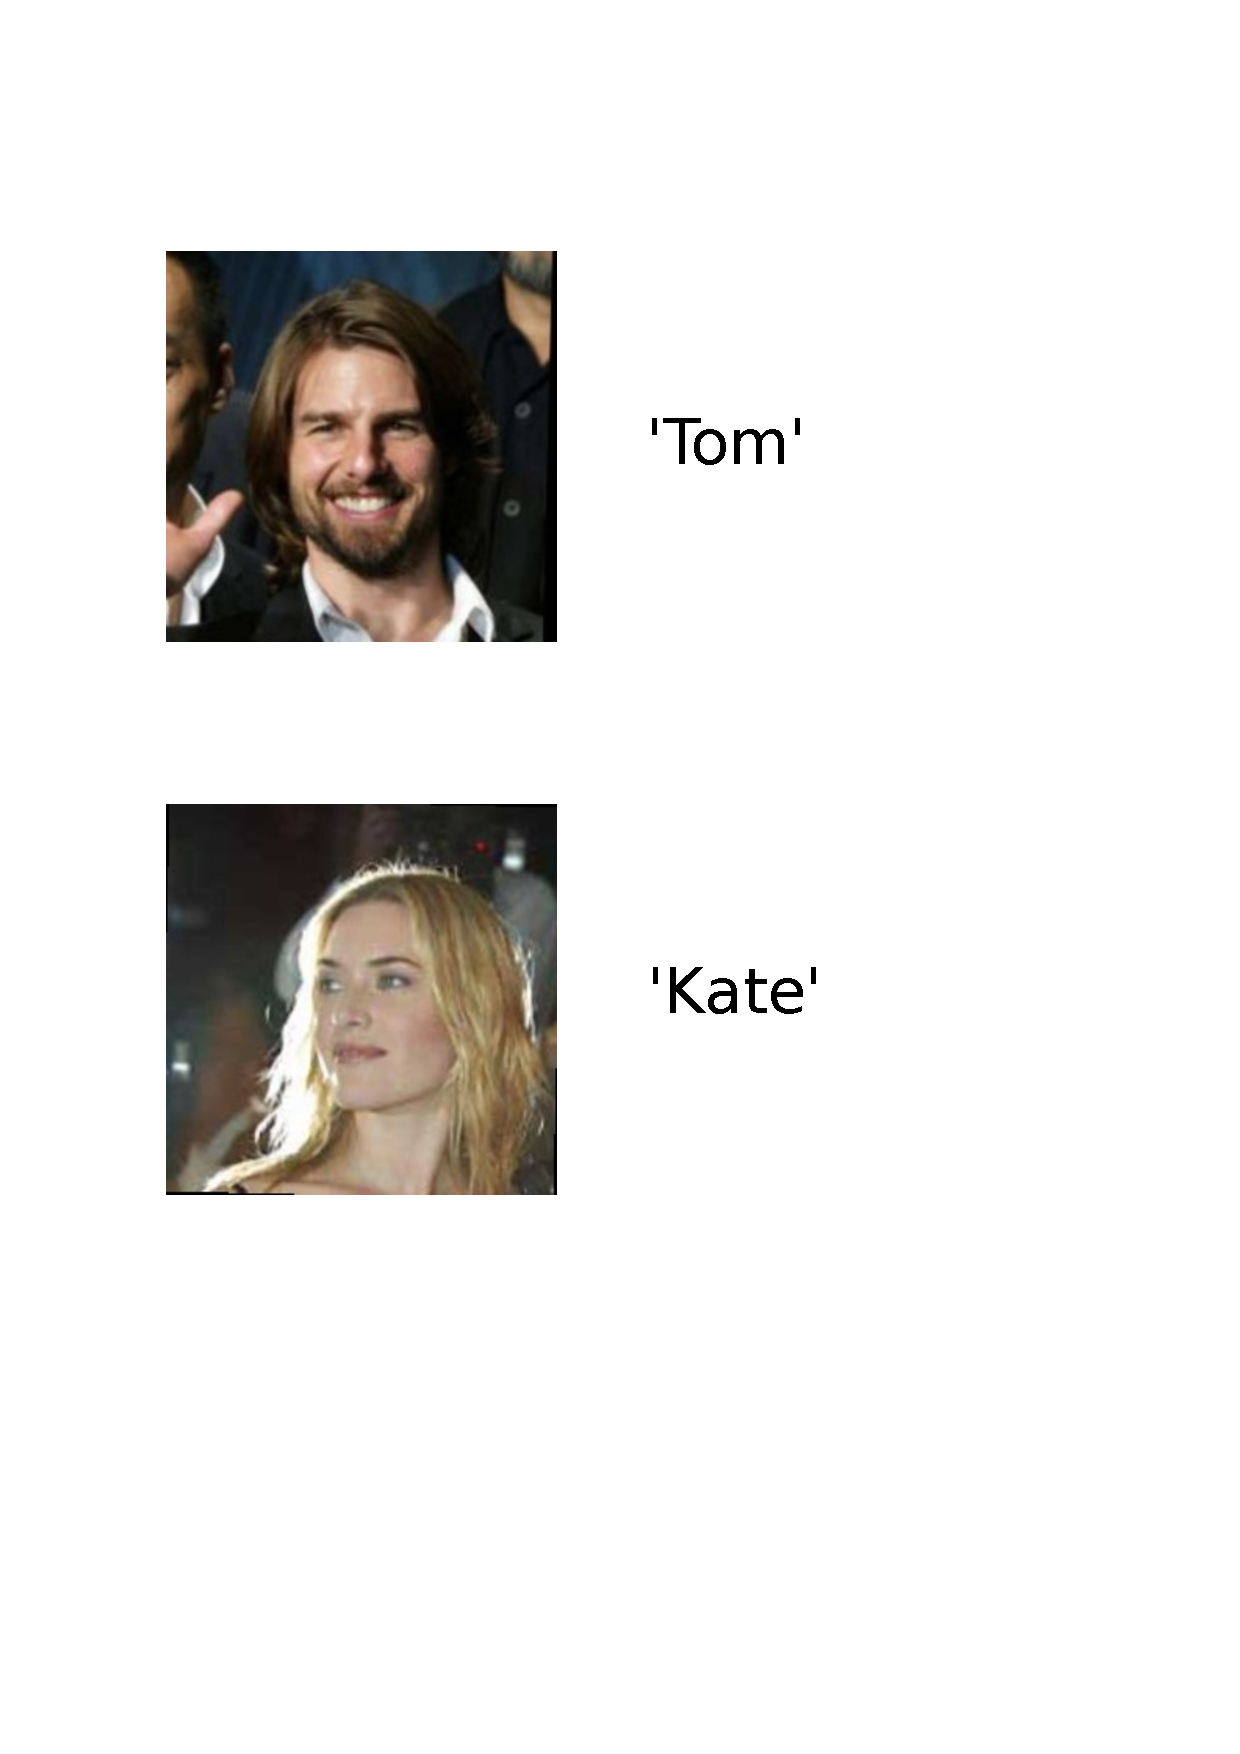
\includegraphics[scale=0.5]{labels.pdf}
%      \label{fig:full}
%   \end{subfigure}
% \begin{subfigure}[b]
% \centering
%      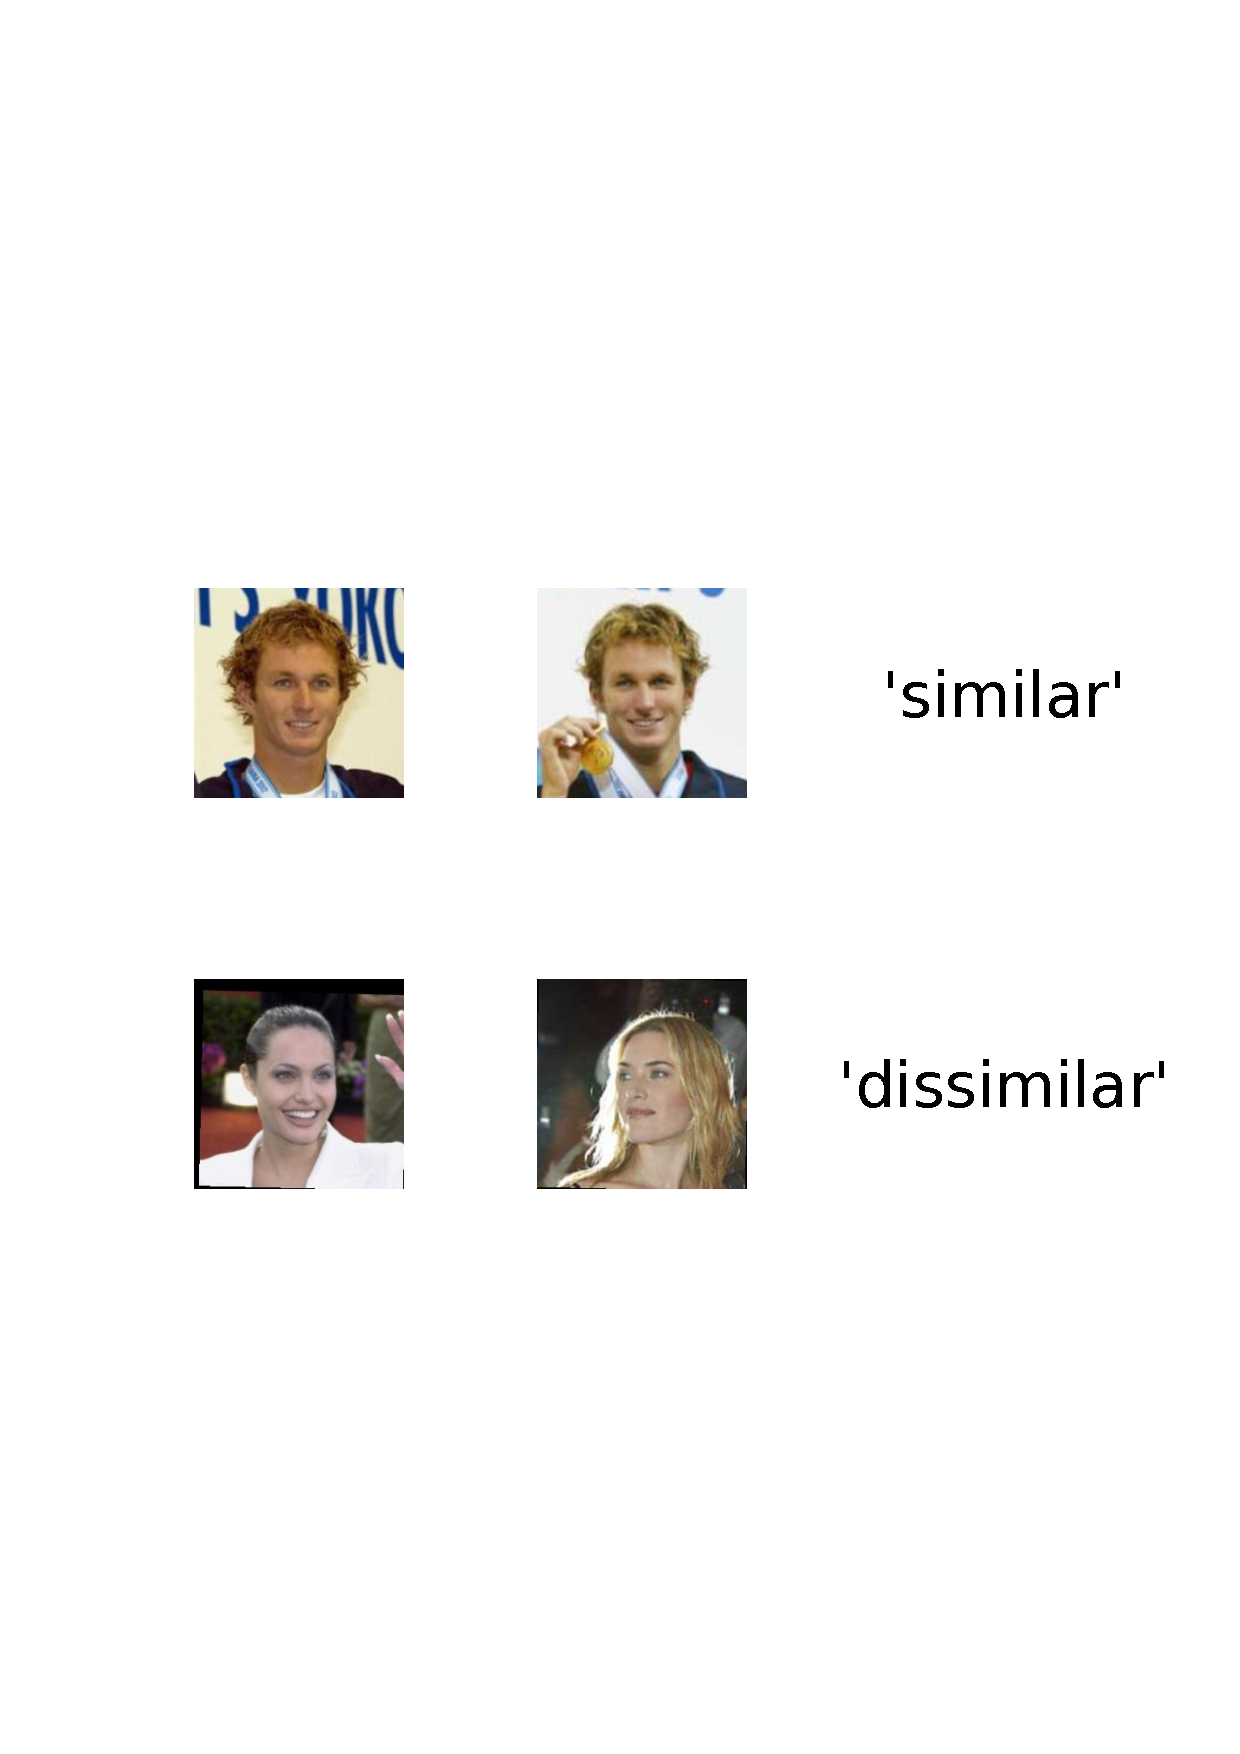
\includegraphics[scale=0.5]{pairs.pdf}
%      \label{fig:pairs}
%   \end{subfigure}
% \begin{subfigure}[b]
% \centering
%      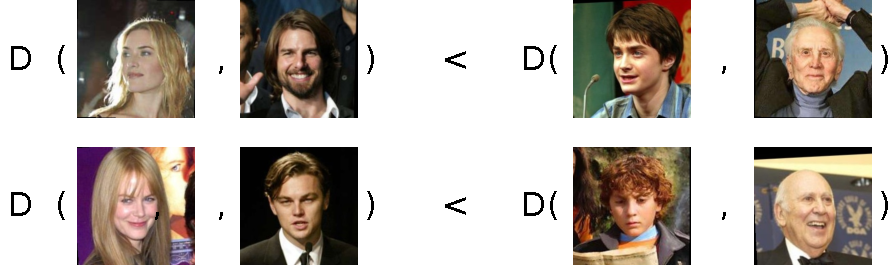
\includegraphics[scale=0.5]{quadruplets.pdf}
%      \label{fig:quadruplets}
%   \end{subfigure}
%   \caption{Different types of supervision for metric learning. (\subref{fig:full}) Full supervision: make samples from the same label (here, identity) closer together than samples from different labels. (\subref{fig:pairs}) Pair supervision: make similar pairs (here, corresponding to the same person) to be closer than dissimilar pairs (different persons). (\subref{fig:quadruplets}) Quadruplet supervision: make the two leftmost samples (here, people of similar age) to be closer than the two rightmost samples (of bigger age difference). Images are taken from the Labeled Faces in the Wild dataset \citep{Huang12}.}
%   \label{fig:contour}
% \end{figure}

%\aurelien{Fig caption is redundant with the main text. could reduce it.}
\section{Overview of the Package}

The current release of \texttt{metric-learn} (v.0.5.0) can be installed from the Python Package Index (PyPI), for Python 2.7 and 3.5 or later. 
The source code is available on GitHub at \url{http://github.com/scikit-learn-contrib/metric-learn} and is free to use, provided under the MIT license. 
\texttt{metric-learn} depends on core libraries from the SciPy ecosystem: \texttt{numpy}, \texttt{scipy}, and \texttt{scikit-learn}.
Detailed documentation (including installation guidelines, the description of the algorithms and the API, as well as examples) is available at \url{http://contrib.scikit-learn.org/metric-learn}.
The development is collaborative and open to all contributors through the usual GitHub workflow of issues and pull requests.
Community interest for the package has been demonstrated by its recent inclusion in the \texttt{scikit-learn-contrib} organization which hosts high-quality \texttt{scikit-learn}-compatible projects,\footnote{\url{https://github.com/scikit-learn-contrib/scikit-learn-contrib}} and by its 1000 stars and 204 forks on GitHub at the time of writing.
The quality of the code is ensured by a thorough test coverage (96\% as of July 2019).
Every new contribution is automatically checked by a continuous integration platform to enforce sufficient test coverage as well as syntax formatting with \texttt{flake8}. %, which allows easy contribution for incoming developers, which can have their code automatically checked.

Currently, \texttt{metric-learn} implements 9 popular metric learning algorithms.
Supervised learners include Neighborhood Components Analysis \citep[NCA,][]{Goldberger04}, Large Margin Nearest Neighbors \citep[LMNN,][]{Weinberger09}, Relative Components Analysis \citep[RCA,][]{Shental02},\footnote{RCA takes as input slightly weaker supervision in the form of \emph{chunklets} (groups of points of same class).} Local Fisher Discriminant Analysis \citep[LFDA,][]{Sugiyama07} and Metric Learning for Kernel Regression \citep[MLKR,][]{Weinberger07}.
The latter is designed for regression problems with continuous labels.
Pair learners include Mahalanobis Metric for Clustering \citep[MMC,][]{Xing2002a}, Information Theoretic Metric Learning \citep[ITML,][]{Davis07} and Sparse High-Dimensional Metric Learning \citep[SDML,][]{Qi09}.
The package implements one quadruplet learner: Metric Learning from Relative Comparisons by Minimizing Squared Residual \citep[LSML,][]{Liu12}. A triplet learner has been recently merged and will be integrated in the next release: Sparse Compositional Metric Learning \citep[SCML,][]{Shi15}.
Detailed descriptions of these algorithms can be found in the package documentation.

\section{Software Architecture and API}

%\aurelien{mention optimization somewhere? rule of thumb opt parameters?}
\texttt{metric-learn} provides a unified interface to all metric learning algorithms. %, including 
%weakly supervised ones (pair and quadruplet learners)
%those whose input format differs from the classic machine learning setting.
It is designed to be fully compatible with the functionality of \texttt{scikit-learn}.
% We briefly explain how the package is structured.
All metric learners inherit from an abstract \texttt{BaseMetricLearner} class, which itself inherits from \texttt{scikit-learn}'s \texttt{BaseEstimator}. All classes inheriting from \texttt{BaseMetricLearner} should implement two methods: \texttt{get\_metric} (returning a function that computes the distance, which can be plugged into \texttt{scikit-learn} estimators like \texttt{KMeansClustering}) and \texttt{score\_pairs} (returning the distances between a set of pairs of points passed as a 3D array).
% \todo[inline]{Should I talk about the classes etc ? Not useful since they are not visible by the user right ?}
% \todo[inline]{I think it can be nice, this is not documentation, but explaining how things are coded}
%\texttt{metric-learn}'s API is designed to be fully compatible with \texttt{scikit-learn} API (\cite{scikit-learn}). 
Mahalanobis distance learning algorithms also inherit from a \texttt{MahalanobisMixin} interface, which has an attribute \texttt{components\_} corresponding to the transformation matrix $L$ of the Mahalanobis distance. \texttt{MahalanobisMixin} implements \texttt{get\_metric} and \texttt{score\_pairs} accordingly as well as a few additional methods. In particular, \texttt{transform} allows to transform data using \texttt{components\_}, and \texttt{get\_mahalanobis\_matrix} returns the Mahalanobis matrix $M=L^TL$.
% This latter can return the mahalanobis matrix with the method \texttt{get\_mahalanobis\_matrix}. Like scikit-learn's algorithms, it can also return a \texttt{components\_} attributes that is the transformation matrix \texttt{L}. Since all these metric learner learn this implicit transformation $L$, they can project the input in the new space using \texttt{transform}. A distance function can also be extracted from them using \texttt{get\_metric}, that can further be used in any scikit-learn estimator like \texttt{KMeansClustering}. They can also return the distance between a dataset of pairs (in the 3D array format (see below), using \texttt{score\_pairs}.

Supervised metric learners inherit from \texttt{scikit-learn}'s base class \texttt{TransformerMixin}, the same base class used by \texttt{sklearn.LinearDiscriminantAnalysis} and others.
As such, they are compatible for pipelining with other estimators via \texttt{sklearn.pipeline.Pipeline}.
% (they pass all scikit-learn's "estimators checks"). 
%  They can easily be pipelined with nearest neighbors estimators to improve their performance: \texttt{better\_knn = sklearn.pipeline.make\_pipeline(NCA(), KNeighborsClassifier())} (TODO: sth to explain NCA is in metric-learn)
% \aurelien{mention pipelining}

% \william{cf. Nathalie's comment: re-introduce weakly supervised metric laerners}
% Algorithms that learn on pairs or quadruplets take as input 3D array of shape \texttt{(n\_samples, t, n\_features)} (where...). In other words, sampling one element along the first dimension returns one tuple (e.g. a pair), that is a matrix of t lines corresponding to the t elements in the tuple.
% This format is what allows all these API choices, since slicing along the 1st dimension
% While a classical input array \texttt{X} in \texttt{scikit-learn} has shape \texttt{(n\_samples, n\_features)}, an array of tuples has shape \texttt{(n\_tuples, t, n\_features)}, where \texttt{t} is the number of elements in a tuple (e.g. 2 for pairs).
% Note that \texttt{scikit-learn} accepts arrays in a broad sense, in what they call "array-like" objects. \texttt{metric-learn} too accepts "tuple-like" objects.
Weakly supervised algorithms (pair, triplet and quadruplet learners) \texttt{fit} and \texttt{predict} on a set of tuples passed as a 3-dimensional array. Tuples can be pairs triplets, or quadruplets depending on the algorithm.
Pair learners take as input an array-like \texttt{pairs} of shape \texttt{(n\_pairs, 2, n\_features)}, as well as an array-like \texttt{y\_pairs} of shape \texttt{(n\_pairs,)} giving labels (similar or dissimilar) for each pair.
In order to \texttt{predict} the labels of new pairs, one needs to set a threshold on the distance value.
This threshold can be set manually or automatically calibrated (at fit time or afterwards on a validation set) to optimize a given score such as accuracy or F1-score using the method \texttt{calibrate\_threshold}.
Triplet learners work on array-like of shape \texttt{(n\_quadruplets, 3, n\_features)}, where for each triplet the second element is the one we want to be closer to the first than the third one.
Quadruplet learners work on array-like of shape \texttt{(n\_quadruplets, 4, n\_features)}, where for each quadruplet the two first elements are the ones we want to be closer than the two last ones. Both triplet and quadruplet learners can naturally \texttt{predict} whether a new triplet/quadruplet is in the right order by comparing the two pairwise distances.
These design choices enable use of \texttt{scikit-learn}'s scoring functions out of the box, as well as the standard routines for model selection, including \texttt{GridSearchCV}.
To illustrate, the following code snippet computes cross validation scores for ITML (with default parameters) on pairs from Labeled Faces in the Wild \citep{Huang12}.
% Also note that for every pair/quadruplet learner, there is a \texttt{\_Supervised} version (e.g. for \texttt{MMC} there is \texttt{MMC\_Supervised}, that is a supervised version that samples pairs of similar samples from intra-class samples, and dissimilar samples from inter-class samples, and fits \texttt{MMC} on these pairs).
\begin{minted}[%linenos=TRUE,
fontsize=\footnotesize]{python}
>>> from sklearn.datasets import fetch_lfw_pairs 
>>> from sklearn.model_selection import cross_validate, train_test_split 
>>> from sklearn.decomposition import PCA 
>>> from metric_learn import ITML 
>>> pairs, y_pairs = [fetch_lfw_pairs()[key] for key in ['pairs', 'target']]
>>> pairs = PCA(n_components=25).fit_transform(pairs.reshape(4400, -1)).reshape(-1, 2, 25) 
>>> pairs, _, y_pairs, _ = train_test_split(pairs, 2*y_pairs-1)  
>>> cross_validate(ITML(), pairs, y_pairs, scoring='roc_auc', return_train_score=True)
\end{minted}
% mmc.predict(pairs)
%\william{warning: the $*\_$ syntax is only compatible in python 3 I think, is it OK ? }
%\aurelien{remove $*\_$, use AUC, maybe remove rescaling, potentially try other weakly sup algo, prior random really useful}
%\aurelien{try to have one import per line if we can make that fit}

% \begin{minted}{python}
% from sklearn.model_selection import GridSearchCV
% model = GridSearchCV(mmc, {'init': ['random', 'identity', 'covariance']})
% model.fit(pairs, y_pairs)
% \end{minted}

\section{Future Work}

\texttt{metric-learn} is under active development. We list here some promising directions to further improve the package. To scale to large datasets, we would like to implement stochastic solvers (SGD and its variants), forming batches of tuples on the fly to avoid loading all data in memory at once. % We would also like to offer better support to inputs in sparse format.
We also plan to incorporate new algorithms that provide added value to the package, in particular some that learn from triplet supervision \citep{Schultz2003a}, can deal with multi-label \citep{liu15} and high-dimensional problems \citep{Liu19}, or learn other forms of metrics \citep[e.g., nonlinear ones, bilinear similarities, and multiple local metrics, see][]{Bellet15}.
%We could also allow metric learn to be used when having multiple labels for each sample, and allow different kind of supervisions, like semi-supervised learning for instance.
%We could also improve the ease of use by adding more examples and adding toy datasets to play with quickly and see the interest of the weaker forms of supervision. About the overall quality of the software, we intend to improve the continuous integration routines, for instance by ensuring a PEP8 syntax checker is run on every pull request, a continuous integration for the documentation.
%\aurelien{if possible, mention algorithms that learn other metrics (similarity, nonlinear, local..}

\acks

We are thankful to Inria for funding 2 years of development. We also thank \texttt{scikit-learn} developers from the Inria Parietal team (in particular Gaël Varoquaux, Alexandre Gramfort and Olivier Grisel) for fruitful discussions on the design of the API and funding to attend SciPy 2019, as well as \texttt{scikit-learn-contrib} reviewers for their valuable feedback.


%  The quality of comparison to previous (if any) related implementations, w.r.t. run-time, memory requirements, features, to explain that significant progress has been made. 

% Manual newpage inserted to improve layout of sample file - not
% needed in general before appendices/bibliography.

\bibliography{metric-learn-jmlr}

\end{document}
